\section{The Qubit}
\label{sec:qubit}

The basic idea behind the implementation of a device for quantum information is realizing a 2-level quantum system.
In the Quantum Device Lab we use superconducting circuits.

\subsection{Quantum LC resonator}

To introduce the implementation of the qubit utilized in our laboratory, we begin by presenting a simplified model: the quantum LC resonator \cite{LC_resonator}.
\begin{figure}
    \begin{minipage}[b]{0.5\linewidth}
      \centering
        

\tikzset{every picture/.style={line width=0.75pt}} %set default line width to 0.75pt        

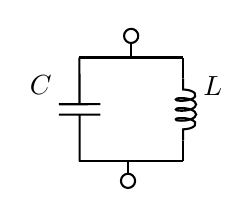
\begin{tikzpicture}[x=0.75pt,y=0.75pt,yscale=-1,xscale=1]
%uncomment if require: \path (0,97); %set diagram left start at 0, and has height of 97

%Shape: Capacitor [id:dp4670171494463129] 
\draw  [line width=0.75]  (50,23.83) -- (50.05,46.33) (60.07,51.31) -- (40.07,51.36) (60.05,46.31) -- (40.05,46.36) (50.07,51.33) -- (50.12,73.83) ;
%Straight Lines [id:da7530368359567341] 
\draw [line width=0.75]    (50,23.83) -- (100,23.83) ;
%Straight Lines [id:da37073903294106214] 
\draw [line width=0.75]    (50,73.83) -- (100,73.83) ;
%Straight Lines [id:da6760299644418128] 
\draw [line width=0.75]    (100,23.83) -- (100,33.83) ;
%Straight Lines [id:da16342394128001536] 
\draw [line width=0.75]    (100,63.83) -- (100,73.83) ;
%Straight Lines [id:da10569605743197075] 
\draw [line width=0.75]    (73.42,79.83) -- (73.42,73.83) ;
%Shape: Circle [id:dp3114709006095975] 
\draw  [line width=0.75]  (70,83.25) .. controls (70,81.36) and (71.53,79.83) .. (73.42,79.83) .. controls (75.3,79.83) and (76.83,81.36) .. (76.83,83.25) .. controls (76.83,85.14) and (75.3,86.67) .. (73.42,86.67) .. controls (71.53,86.67) and (70,85.14) .. (70,83.25) -- cycle ;
%Straight Lines [id:da44379321850243414] 
\draw [line width=0.75]    (75,16.83) -- (75,23.83) ;
%Shape: Circle [id:dp37786908957841614] 
\draw  [line width=0.75]  (78.33,13.33) .. controls (78.38,15.22) and (76.89,16.78) .. (75,16.83) .. controls (73.11,16.88) and (71.55,15.39) .. (71.5,13.5) .. controls (71.45,11.62) and (72.94,10.05) .. (74.83,10) .. controls (76.71,9.95) and (78.28,11.44) .. (78.33,13.33) -- cycle ;
%Shape: Inductor (Air Core) [id:dp009772684946594334] 
\draw   (100,33.83) -- (100,39.23) .. controls (102.63,39.31) and (104.87,40.06) .. (105.66,41.12) .. controls (106.44,42.18) and (105.61,43.34) .. (103.55,44.03) .. controls (101.95,44.57) and (99.88,44.79) .. (97.87,44.63) .. controls (97.08,44.63) and (96.45,44.36) .. (96.45,44.03) .. controls (96.45,43.7) and (97.08,43.43) .. (97.87,43.43) .. controls (99.88,43.28) and (101.95,43.5) .. (103.55,44.03) .. controls (105.26,44.66) and (106.23,45.52) .. (106.23,46.43) .. controls (106.23,47.34) and (105.26,48.21) .. (103.55,48.83) .. controls (101.95,49.37) and (99.88,49.59) .. (97.87,49.43) .. controls (97.08,49.43) and (96.45,49.16) .. (96.45,48.83) .. controls (96.45,48.5) and (97.08,48.23) .. (97.87,48.23) .. controls (99.88,48.08) and (101.95,48.3) .. (103.55,48.83) .. controls (105.26,49.46) and (106.23,50.32) .. (106.23,51.23) .. controls (106.23,52.14) and (105.26,53.01) .. (103.55,53.63) .. controls (101.95,54.17) and (99.88,54.39) .. (97.87,54.23) .. controls (97.08,54.23) and (96.45,53.96) .. (96.45,53.63) .. controls (96.45,53.3) and (97.08,53.03) .. (97.87,53.03) .. controls (99.88,52.88) and (101.95,53.1) .. (103.55,53.63) .. controls (105.61,54.33) and (106.44,55.48) .. (105.66,56.54) .. controls (104.87,57.61) and (102.63,58.35) .. (100,58.43) -- (100,63.83) ;

% Text Node
\draw (108.23,43.43) node [anchor=south west] [inner sep=0.75pt]   [align=left] {$\displaystyle L$};
% Text Node
\draw (38.05,43.36) node [anchor=south east] [inner sep=0.75pt]   [align=left] {$\displaystyle C$};


\end{tikzpicture}
        \vspace{-0.7cm}
        \caption{Circuit diagram of LC resonator}
        \label{fig:LC}
    \end{minipage}
    \hfill
    \begin{minipage}[b]{0.45\linewidth}
      \centering
      

\tikzset{every picture/.style={line width=0.75pt}} %set default line width to 0.75pt        

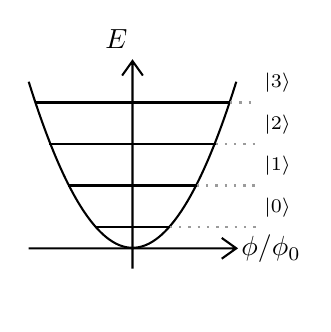
\begin{tikzpicture}[x=0.75pt,y=0.75pt,yscale=-1,xscale=1]
%uncomment if require: \path (0,200); %set diagram left start at 0, and has height of 200

%Shape: Parabola [id:dp37890511708987873] 
\draw   (60,70) .. controls (93.33,176.67) and (126.67,176.67) .. (160,70) ;
%Shape: Axis 2D [id:dp3773695523891737] 
\draw  (60,150.25) -- (160,150.25)(110,60) -- (110,160) (153,145.25) -- (160,150.25) -- (153,155.25) (105,67) -- (110,60) -- (115,67)  ;
%Straight Lines [id:da3077075366408746] 
\draw    (92,140) -- (128,140) ;
%Straight Lines [id:da2626121978197561] 
\draw    (79,120) -- (141,120) ;
%Straight Lines [id:da8498237157026597] 
\draw    (70,100) -- (150,100) ;
%Straight Lines [id:da16494940971997396] 
\draw    (63,80) -- (157,80) ;
%Straight Lines [id:da15643784358380952] 
\draw [color={rgb, 255:red, 155; green, 155; blue, 155 }  ,draw opacity=1 ] [dash pattern={on 0.84pt off 2.51pt}]  (128,140) -- (170,140) ;
%Straight Lines [id:da7225933392434986] 
\draw [color={rgb, 255:red, 155; green, 155; blue, 155 }  ,draw opacity=1 ] [dash pattern={on 0.84pt off 2.51pt}]  (141,120) -- (170,120) ;
%Straight Lines [id:da6235512774693245] 
\draw [color={rgb, 255:red, 155; green, 155; blue, 155 }  ,draw opacity=1 ] [dash pattern={on 0.84pt off 2.51pt}]  (150,100) -- (170,100) ;
%Straight Lines [id:da04257430271569573] 
\draw [color={rgb, 255:red, 155; green, 155; blue, 155 }  ,draw opacity=1 ] [dash pattern={on 0.84pt off 2.51pt}]  (157,80) -- (170,80) ;

% Text Node
\draw (109,49.5) node [anchor=east] [inner sep=0.75pt]   [align=left] {$\displaystyle E$};
% Text Node
\draw (161,142.4) node [anchor=north west][inner sep=0.75pt]    {$\phi /\phi _{0}$};
% Text Node
\draw (172,136.6) node [anchor=south west] [inner sep=0.75pt]  [font=\scriptsize]  {$| 0\rangle $};
% Text Node
\draw (172,116.6) node [anchor=south west] [inner sep=0.75pt]  [font=\scriptsize]  {$| 1\rangle $};
% Text Node
\draw (172,96.6) node [anchor=south west] [inner sep=0.75pt]  [font=\scriptsize]  {$| 2\rangle $};
% Text Node
\draw (172,76.6) node [anchor=south west] [inner sep=0.75pt]  [font=\scriptsize]  {$| 3\rangle $};


\end{tikzpicture}
      \vspace{-1.5cm}
      \caption{Energy spectrum of LC resonator}
      \label{fig:Energy_spectrum}
    \end{minipage}
  \end{figure}
The circuit diagram is illustrated in \cref{fig:LC}, depicting a system that emulates the behavior of a quantum oscillator.
In classical physics, the Hamiltonian for a harmonic oscillator is expressed as follows:
\begin{equation}
    H = \frac{\phi^2}{2L} + \frac{Q^2}{2C},
\end{equation}
where $\phi$ represents the flux in the inductor, and $Q$ denotes the charge on the capacitor.

Quantizing this classical Hamiltonian involves replacing $\phi$ and $Q$ with the flux operator ($\hat{\phi}$) and charge operator ($\hat{Q}$), respectively.
The resulting quantum Hamiltonian, expressed in second quantization form, is given by:
\begin{equation}
    \hat{H} = \frac{\hat{\phi}^2}{2L} + \frac{\hat{Q}^2}{2C} = \hbar \omega \left(\hat{a}^\dagger \hat{a} + \frac{1}{2}\right),
\end{equation}
where $\omega = 1/\sqrt{LC}$ is the resonance frequency of the circuit.
The operators $\hat{a}^\dagger$ and $\hat{a}$ correspond to the creation and annihilation operators of excitations, respectively. 
In this scenario, the excitations represent the difference in the number of charges between the two plates of the capacitor.
Utilizing this quantum description of the LC circuit, we obtain the energy spectrum illustrated in \cref{fig:Energy_spectrum} ($\phi_0 = h/2e$ is the flux quantum) .
The quantization of energy levels in relation to the magnetic flux $\phi$ is clearly evident in the figure.

\subsection{The transmon resonator}

The issue of energy level harmonicity poses a challenge when aiming to construct a quantum processor. 
In this context, determining the specific transitions being driven becomes uncertain, as the energy differences between consecutive levels remain identical.
To address this, we introduce non-linearity into our circuit through the incorporation of the Josephson junction \cite{JOSEPHSON}.

Josephson demonstrated that a current without dissipation could flow between two superconducting electrodes when separated by a thin insulating barrier. Specifically, he established that this supercurrent is determined by
\begin{equation}
    I = I_c \sin(\varphi),
\end{equation}
where $I_c$ represents the critical current of the junction, and $\varphi$ denotes the phase difference between the superconducting condensates on each side of the junction.
\begin{figure}
    \begin{minipage}[b]{0.5\linewidth}
      \centering
        

\tikzset{every picture/.style={line width=0.75pt}} %set default line width to 0.75pt        

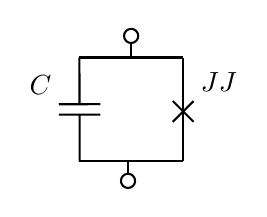
\begin{tikzpicture}[x=0.75pt,y=0.75pt,yscale=-1,xscale=1]
%uncomment if require: \path (0,97); %set diagram left start at 0, and has height of 97

%Shape: Capacitor [id:dp8072216489364277] 
\draw  [line width=0.75]  (60,23.83) -- (60.05,46.33) (70.07,51.31) -- (50.07,51.36) (70.05,46.31) -- (50.05,46.36) (60.07,51.33) -- (60.12,73.83) ;
%Straight Lines [id:da183774352314787] 
\draw [line width=0.75]    (105,54.83) -- (115,44.83) ;
%Straight Lines [id:da1896922658483372] 
\draw [line width=0.75]    (105,44.83) -- (115,54.83) ;

%Straight Lines [id:da33699096520016336] 
\draw [line width=0.75]    (60,23.83) -- (110,23.83) ;
%Straight Lines [id:da6915014186556621] 
\draw [line width=0.75]    (60,73.83) -- (110,73.83) ;
%Straight Lines [id:da36159548727595725] 
\draw [line width=0.75]    (83.42,79.83) -- (83.42,73.83) ;
%Shape: Circle [id:dp8015144235751568] 
\draw  [line width=0.75]  (80,83.25) .. controls (80,81.36) and (81.53,79.83) .. (83.42,79.83) .. controls (85.3,79.83) and (86.83,81.36) .. (86.83,83.25) .. controls (86.83,85.14) and (85.3,86.67) .. (83.42,86.67) .. controls (81.53,86.67) and (80,85.14) .. (80,83.25) -- cycle ;
%Straight Lines [id:da3714464315940995] 
\draw [line width=0.75]    (85,16.83) -- (85,23.83) ;
%Shape: Circle [id:dp25364190410803145] 
\draw  [line width=0.75]  (88.33,13.33) .. controls (88.38,15.22) and (86.89,16.78) .. (85,16.83) .. controls (83.11,16.88) and (81.55,15.39) .. (81.5,13.5) .. controls (81.45,11.62) and (82.94,10.05) .. (84.83,10) .. controls (86.71,9.95) and (88.28,11.44) .. (88.33,13.33) -- cycle ;
%Straight Lines [id:da8131700138845456] 
\draw    (110,23.83) -- (110,73.83) ;

% Text Node
\draw (48.05,43.36) node [anchor=south east] [inner sep=0.75pt]   [align=left] {$\displaystyle C$};
% Text Node
\draw (117,41.83) node [anchor=south west] [inner sep=0.75pt]   [align=left] {$\displaystyle JJ$};


\end{tikzpicture}
        \vspace{-0.8cm}
        \caption{Circuit diagram of a transmon resonator}
        \label{fig:JJ_circuit}
    \end{minipage}
    \hfill
    \begin{minipage}[b]{0.45\linewidth}
      \centering
      

\tikzset{every picture/.style={line width=0.75pt}} %set default line width to 0.75pt        

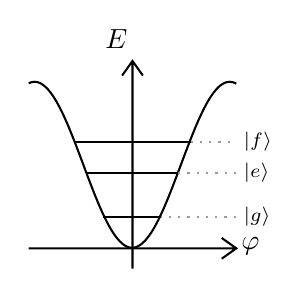
\begin{tikzpicture}[x=0.75pt,y=0.75pt,yscale=-1,xscale=1]
%uncomment if require: \path (0,200); %set diagram left start at 0, and has height of 200

%Straight Lines [id:da03495800698048135] 
\draw [color={rgb, 255:red, 155; green, 155; blue, 155 }  ,draw opacity=1 ] [dash pattern={on 0.84pt off 2.51pt}]  (123,135) -- (160,135) ;
%Shape: Axis 2D [id:dp2373273044965445] 
\draw  (60,150.25) -- (160,150.25)(110,60) -- (110,160) (153,145.25) -- (160,150.25) -- (153,155.25) (105,67) -- (110,60) -- (115,67)  ;
%Shape: Wave [id:dp12933752750229321] 
\draw   (60,70.71) .. controls (60.93,70.25) and (61.87,70) .. (62.82,70) .. controls (71.32,70) and (78.66,89.51) .. (86.32,110) .. controls (93.98,130.49) and (101.32,150) .. (109.82,150) .. controls (118.32,150) and (125.66,130.49) .. (133.32,110) .. controls (140.98,89.51) and (148.32,70) .. (156.82,70) .. controls (157.9,70) and (158.96,70.31) .. (160,70.9) ;
%Straight Lines [id:da530045401686506] 
\draw    (96,135) -- (123,135) ;
%Straight Lines [id:da34934240050097976] 
\draw    (88,114) -- (132,114) ;
%Straight Lines [id:da19311872891258342] 
\draw    (82,99) -- (138,99) ;
%Straight Lines [id:da3065730660397551] 
\draw [color={rgb, 255:red, 155; green, 155; blue, 155 }  ,draw opacity=1 ] [dash pattern={on 0.84pt off 2.51pt}]  (132,114) -- (160,114) ;
%Straight Lines [id:da057644743938617404] 
\draw [color={rgb, 255:red, 155; green, 155; blue, 155 }  ,draw opacity=1 ] [dash pattern={on 0.84pt off 2.51pt}]  (138,99) -- (160,99) ;

% Text Node
\draw (109,49.5) node [anchor=east] [inner sep=0.75pt]   [align=left] {$\displaystyle E$};
% Text Node
\draw (161,143.4) node [anchor=north west][inner sep=0.75pt]    {$\varphi $};
% Text Node
\draw (162,135) node [anchor=west] [inner sep=0.75pt]  [font=\scriptsize]  {$|g\rangle $};
% Text Node
\draw (162,114) node [anchor=west] [inner sep=0.75pt]  [font=\scriptsize]  {$|e\rangle $};
% Text Node
\draw (162,99) node [anchor=west] [inner sep=0.75pt]  [font=\scriptsize]  {$|f\rangle $};


\end{tikzpicture}
      \vspace{-1.2cm}
      \caption{Energy spectrum of transmon resonator}
      \label{fig:Energy_spectrum_JJ}
    \end{minipage}
  \end{figure}

By replacing the inductor of the LC resonator with a Josephson junction (\cref{fig:JJ_circuit}), we achieve the desired anharmonicity of the energy levels.
The resulting potential becomes a cosine potential, leading to non-equidistant energy levels, as illustrated in \cref{fig:Energy_spectrum_JJ}.
To gain a deeper insight into the origin of this anharmonicity, we present the Hamiltonian of the Josephson junction resonator in second quantization formalism:
\begin{equation}
\label{eq:cosina_H}
    \hat{H} = 
    \hbar \omega \hat{a}^\dagger \hat{a} - 
    \frac{E_C}{2}\hat{a}^\dagger\hat{a}^\dagger\hat{a}\hat{a} ,
\end{equation}
where
\begin{equation}
    E_C = \frac{e^2}{2 C_\Sigma}
\end{equation} 
is the charging energy and $C_\Sigma = C_J + C_C$ is the total capacitance.
The Hamiltonian described in \cref{eq:cosina_H} essentially represents an harmonic oscillator incorporating an anharmonicity correction. 
This allows us to address individual energy levels separately.

This arrangement is employed in quantum computation, utilizing the first two energy levels, $\ket{g}$ and $\ket{e}$, for encoding quantum state information. 
Typically, the $\ket{f}$ state is utilized as an auxiliary energy level during the implementation of certain operations.

In our laboratory, the transmon qubit is realized through the Josephson junction resonator under specific conditions known as the \emph{transmon regime} \cite{transmon_regime}.

An advantageous adaptation of the transmon artificial atom is the flux-tunable transmon, in which the single Josephson junction is substituted with two parallel junctions, forming a superconducting quantum interference device (SQUID).
\begin{figure}
    \begin{minipage}[b]{0.5\linewidth}
      \centering
      


\tikzset{every picture/.style={line width=0.75pt}} %set default line width to 0.75pt        

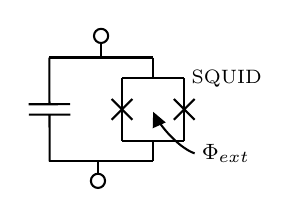
\begin{tikzpicture}[x=0.75pt,y=0.75pt,yscale=-1,xscale=1]
%uncomment if require: \path (0,97); %set diagram left start at 0, and has height of 97

%Shape: Capacitor [id:dp34366919102472526] 
\draw  [line width=0.75]  (20,23.83) -- (20.05,46.33) (30.07,51.31) -- (10.07,51.36) (30.05,46.31) -- (10.05,46.36) (20.07,51.33) -- (20.12,73.83) ;
%Straight Lines [id:da9532858123226031] 
\draw [line width=0.75]    (55,33.83) -- (85,33.83) ;
%Straight Lines [id:da4790035249190253] 
\draw [line width=0.75]    (85,33.83) -- (85,63.83) ;
%Straight Lines [id:da5192559786668693] 
\draw [line width=0.75]    (55,33.83) -- (55,63.83) ;
%Straight Lines [id:da23389027703175358] 
\draw [line width=0.75]    (55,63.83) -- (85,63.83) ;
%Straight Lines [id:da6028752523424945] 
\draw [line width=0.75]    (50,43.83) -- (60,53.83) ;
%Straight Lines [id:da22268293223346158] 
\draw [line width=0.75]    (50,53.83) -- (60,43.83) ;
%Straight Lines [id:da7666685944565205] 
\draw [line width=0.75]    (80,53.83) -- (90,43.83) ;
%Straight Lines [id:da0860971350076063] 
\draw [line width=0.75]    (80,43.83) -- (90,53.83) ;
%Straight Lines [id:da32147396047949894] 
\draw [line width=0.75]    (20,23.83) -- (70,23.83) ;
%Straight Lines [id:da3842851758264739] 
\draw [line width=0.75]    (20,73.83) -- (70,73.83) ;
%Straight Lines [id:da04257544936461244] 
\draw [line width=0.75]    (70,23.83) -- (70,33.83) ;
%Straight Lines [id:da22754146049716317] 
\draw [line width=0.75]    (70,63.83) -- (70,73.83) ;
%Straight Lines [id:da6459112049306985] 
\draw [line width=0.75]    (43.42,79.83) -- (43.42,73.83) ;
%Shape: Circle [id:dp6531205659740902] 
\draw  [line width=0.75]  (40,83.25) .. controls (40,81.36) and (41.53,79.83) .. (43.42,79.83) .. controls (45.3,79.83) and (46.83,81.36) .. (46.83,83.25) .. controls (46.83,85.14) and (45.3,86.67) .. (43.42,86.67) .. controls (41.53,86.67) and (40,85.14) .. (40,83.25) -- cycle ;
%Straight Lines [id:da42435820900303667] 
\draw [line width=0.75]    (45,16.83) -- (45,23.83) ;
%Shape: Circle [id:dp32456243319283773] 
\draw  [line width=0.75]  (48.33,13.33) .. controls (48.38,15.22) and (46.89,16.78) .. (45,16.83) .. controls (43.11,16.88) and (41.55,15.39) .. (41.5,13.5) .. controls (41.45,11.62) and (42.94,10.05) .. (44.83,10) .. controls (46.71,9.95) and (48.28,11.44) .. (48.33,13.33) -- cycle ;

%Curve Lines [id:da7487363329577509] 
\draw [color={rgb, 255:red, 0; green, 0; blue, 0 }  ,draw opacity=1 ]   (90,70) .. controls (83.25,67.65) and (75.22,59.11) .. (71.34,52.55) ;
\draw [shift={(70,50)}, rotate = 65.77] [fill={rgb, 255:red, 0; green, 0; blue, 0 }  ,fill opacity=1 ][line width=0.08]  [draw opacity=0] (7.14,-3.43) -- (0,0) -- (7.14,3.43) -- cycle    ;

% Text Node
\draw (87,33.83) node [anchor=west] [inner sep=0.75pt]   [align=left] {{\scriptsize SQUID}};
% Text Node
\draw (92,70) node [anchor=west] [inner sep=0.75pt]  [font=\footnotesize,color={rgb, 255:red, 0; green, 0; blue, 0 }  ,opacity=1 ] [align=left] {$\displaystyle \Phi _{\text{ext}}$};


\end{tikzpicture}
      \captionsetup{skip=-20pt}
      \caption{Circuit diagram of a flux-tunable transmon}
      \label{fig:transmon_circuit}
    \end{minipage}
    \hfill
    \begin{minipage}[b]{0.45\linewidth}
      \centering
      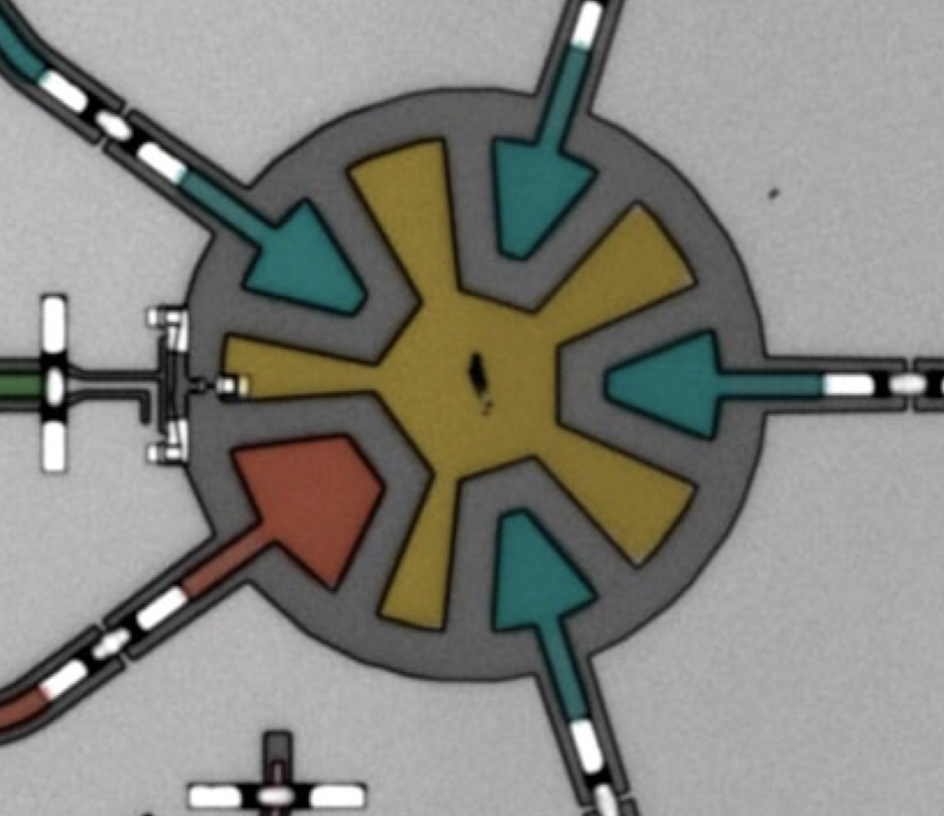
\includegraphics[width = 0.5 \textwidth]{Images/Chap1/star_transmon.png}
      \caption{Star-shaped transmon qubit}
      \label{fig:star_transmon}
    \end{minipage}
  \end{figure}

Replacing the Josephson junction with a SQUID loop introduces a flux-dependent Josephson energy, $E_J(\Phi_\text{ext})$ (see \cref{fig:transmon_circuit}).
Consequently, this results in a flux-tunable transmon frequency 
\begin{equation}
    \omega_q(\Phi_\text{ext}) = \sqrt{8 E_C|E_J(\Phi_\text{ext})|} - E_C/\hbar^3.
\end{equation}
In practical terms, the transmon frequency can be dynamically tuned by up to $\SI{1}{\giga\hertz}$ \cite{di_carlo}.
The magnetic flux within the SQUID loop is produced and regulated by the current flowing through the \emph{flux line}, a nearby waveguide adjacent to the SQUID loop.

In our laboratory, we employ star-shaped transmon qubits \cite{transmon_qubits}, similar to the one depicted in \cref{fig:star_transmon}.
These qubits feature a SQUID loop, making them flux tunable.



